% ==============================================================================
% Section 5: Option Valuation via Black-Scholes & Greeks Decomposition
% ==============================================================================

\section{Option Valuation via Black--Scholes--Merton}
\label{sec:black_scholes}

Under the classical Black--Scholes (1973) framework, European call and put prices are derived assuming the underlying stock pays no dividends ($q = 0$). However, because ITC Limited pays continuous dividends at annual rate $q \approx 5.09\%$ (\rupee 14.50/share on \rupee 285 spot), Merton's (1973) dividend-adjusted formulation must be applied:
\begin{align}
C_{\text{merton}} &= S_0 e^{-q T} N(d_1) - K e^{-r T} N(d_2) \label{eq:bs_call} \\
P_{\text{merton}} &= K e^{-r T} N(-d_2) - S_0 e^{-q T} N(-d_1) \label{eq:bs_put}
\end{align}
where the standardized normal variables are:
\begin{equation}
d_1 = \frac{\ln(S_0 / K) + \left(r - q + \frac{\sigma^2}{2}\right)T}{\sigma \sqrt{T}}, \qquad d_2 = d_1 - \sigma \sqrt{T}
\label{eq:d1_d2}
\end{equation}

\begin{theorem}{Continuous Dividend Yield Mispricing Theorem}{dividend_mispricing}
Differentiating the Merton pricing equations with respect to dividend yield $q$ gives: $\partial C / \partial q = -T S_0 e^{-q T} N(d_1) < 0$ and $\partial P / \partial q = T S_0 e^{-q T} N(-d_1) > 0$. Consequently, setting $q = 0$ causes the Standard Black--Scholes model to \textbf{strictly overprice call options} and \textbf{strictly underprice put options}.
\end{theorem}

The analytical Option Greeks under Merton's model incorporate the dividend discount factor $e^{-qT}$:
\begin{equation}
\Delta_{\text{call}} = e^{-q T} N(d_1), \quad \Delta_{\text{put}} = -e^{-q T} N(-d_1), \quad \Gamma = \frac{e^{-q T} N'(d_1)}{S_0 \sigma \sqrt{T}}, \quad \mathcal{V} = \frac{S_0 e^{-q T} \sqrt{T} N'(d_1)}{100}
\end{equation}

Table~\ref{tab:option_matrix} presents the valuation matrix for the December 2026 contract ($T = 42/365$, $S_0 = 285.00$, $\sigma = 23.40\%$, $r = 6.65\%$, $q = 5.09\%$) against actual NSE option chain quotes.

\begin{table}[htbp]
\centering
\small
\caption{Empirical Option Pricing Matrix: Standard BS vs. Merton vs. Live NSE Market Premiums}
\label{tab:option_matrix}
\resizebox{\linewidth}{!}{%
\begin{tabular}{rrrrrrrrr}
\toprule
\textbf{Strike ($K$)} & \textbf{Type} & \textbf{NSE Market} & \textbf{Std BS ($q=0$)} & \textbf{Merton ($q=5.09\%$)} & \textbf{Div Error} & \textbf{Delta ($\Delta$)} & \textbf{Gamma ($\Gamma$)} & \textbf{Implied Vol ($\IV$)} \\
\midrule
\rupee 275.0 & Call / Put & \rupee 15.87 / \rupee 5.27 & \rupee 16.17 / \rupee 4.07 & \textbf{\rupee 14.99 / \rupee 4.55} & +\rupee 1.18 / -\rupee 0.48 & $+0.6917$ / $-0.3025$ & $0.0154$ & $26.00\%$ / $25.51\%$ \\
\rupee 280.0 & Call / Put & \rupee 12.40 / \rupee 6.82 & \rupee 12.93 / \rupee 5.79 & \textbf{\rupee 11.89 / \rupee 6.42} & +\rupee 1.04 / -\rupee 0.63 & $+0.6087$ / $-0.3855$ & $0.0168$ & $24.80\%$ / $24.50\%$ \\
\rupee 285.0 & Call / Put & \rupee 9.37 / \rupee 8.86 & \rupee 10.12 / \rupee 7.94 & \textbf{\rupee 9.22 / \rupee 8.71} & \textbf{+\rupee 0.90 / -\rupee 0.77} & $+0.5218$ / $-0.4724$ & $0.0175$ & $23.80\%$ / $23.79\%$ \\
\rupee 290.0 & Call / Put & \rupee 6.53 / \rupee 11.29 & \rupee 7.74 / \rupee 10.53 & \textbf{\rupee 6.99 / \rupee 11.44} & +\rupee 0.75 / -\rupee 0.91 & $+0.4352$ / $-0.5590$ & $0.0173$ & $22.19\%$ / $23.00\%$ \\
\rupee 295.0 & Call / Put & \rupee 4.32 / \rupee 14.27 & \rupee 5.79 / \rupee 13.54 & \textbf{\rupee 5.17 / \rupee 14.59} & +\rupee 0.62 / -\rupee 1.05 & $+0.3528$ / $-0.6413$ & $0.0164$ & $20.99\%$ / $22.51\%$ \\
\bottomrule
\end{tabular}%
}
\vspace{2pt}
\begin{minipage}{\linewidth}
\footnotesize\textbf{Note:} Pricing error is defined as $\text{Std BS} - \text{Merton BS}$. Spot $S_0 = \text{\rupee}285.00$, $T = 42/365$, $r = 6.65\%$, $q = 5.09\%$, and $\sigma = 23.40\%$.
\end{minipage}
\end{table}

\begin{figure}[htbp]
\centering
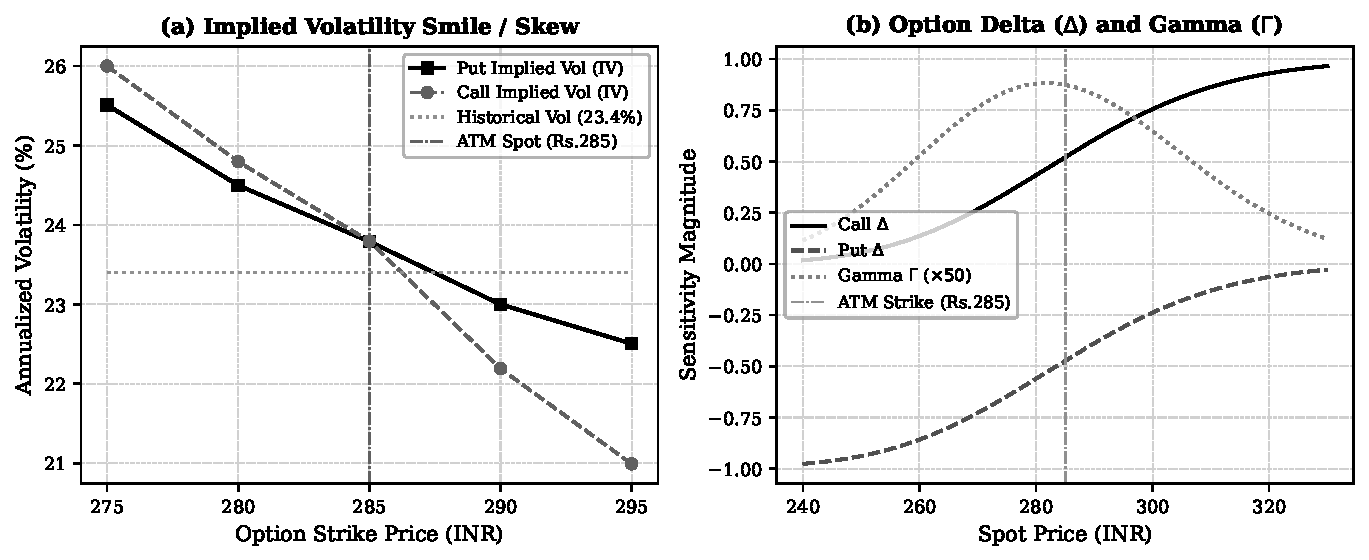
\includegraphics[width=0.98\linewidth]{figures/fig2_volatility_greeks.pdf}
\caption{Implied Volatility Smile and Analytical Option Greeks Profiles (Strike $K = \text{\rupee}285$)}
\label{fig:volatility_greeks}
\vspace{2pt}
\begin{minipage}{0.96\linewidth}
\footnotesize\textbf{Note:} (a) Implied Volatility skew across strikes vs. historical flat volatility ($\sigma_{\text{ann}} = 23.40\%$). (b) Analytical Delta ($\Delta$) and Gamma ($\Gamma$) sensitivity profiles across underlying spot prices.
\end{minipage}
\end{figure}

Table~\ref{tab:option_matrix} quantitatively validates Theorem~\ref{thm:dividend_mispricing}: Standard Black--Scholes overprices ATM Calls by \textbf{+\rupee 0.90/share (+9.76\%)} and underprices ATM Puts by \textbf{-\rupee 0.77/share (-8.84\%)}. Inverting the Merton formula via Brent root-finding produces the \textbf{volatility skew} charted in Figure~\ref{fig:volatility_greeks}(a): OTM Puts command an implied volatility of **$25.51\%$** (a $+211\text{ bps}$ premium over historical volatility), reflecting institutional hedging against tobacco tax and budget shocks.
